\chapter{Motivatie en Uitdagingen}
% TODO?
\label{hoofdstuk:motivatie}
Dit hoofdstuk behandelt de motivatie voor dit onderwerp, de uitdagingen die vermeldenswaardig zijn bij de zoektocht naar een gepaste oplossing en het plan van aanpak voor de oplossing.

\section{Motivatie}

\begin{figure}
    \centering
    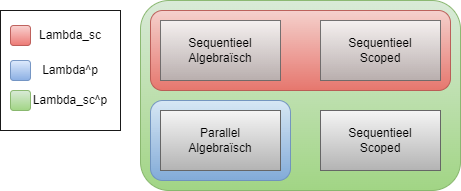
\includegraphics[width=\textwidth]{Media/scope.png}
    \caption{Scope van de verschillende calculi vermeld in deze thesis}
    \label{fig:motiv}
\end{figure}

De primaire motivatie voor de ontwikkeling van de calculus is het ontbreken van een calculus die zowel parallelle als sequentiële uitvoering van zowel algebraïsche als scoped effecten in de literatuur. De $\lambda_{sc}$-calculus \cite{Bosman2022} ondersteunt sequentiële uitvoering van algebraïsche en scoped effecten. De $\lambda^{p}$-calculus ondersteunt parallelle uitvoering van algebraïsche effecten. Het doel van de $\lambda_{sc}^{p}$-calculus is om deze leemte in de literatuur te vullen en zowel parallelle als sequentiële uitvoering van algebraïsche en scoped effecten mogelijk te maken zoals afgebeeld in Figuur \ref{fig:motiv}. \newline
De manier van parallelle uitvoering is zoals uitgewerkt in de $\lambda^p$-calculus, namelijk het opstellen van een nieuw effect of een nieuwe constructie die een lijst van inputs geeft en eenzelfde computatie in parallel uitvoert voor elke input in de lijst. 

\section{Syntaxis}
De syntaxis van de $\lambda^p$-calculus verdeelt de termen in expressies in handlers terwijl die van de $\lambda_{sc}$-calculus de termen verdeelt in waarden en computaties. De gecombineerde calculus houdt de laatste conventie aan en syntactische uitbreidingen voor parallelle uitvoering van de $\lambda^p$-calculus moeten aangepast worden naar deze conventie.

\section{Operationele semantiek}
De $\lambda^p$-calculus modelleert geen complete, klein-stappige operationele semantiek. De semantiek kan in huidige vorm niet ingepast worden in de $\lambda_{sc}$-calculus en zal de introductie en eigen contributie van meerdere nieuwe regels noodzaken om in een klein-stappige operationele semantiek te passen.

\section{Type- en Effect-Systeem}
De $\lambda^p$-calculus heeft geen type- en effect-systeem. De gecombineerde calculus bouwt verder op het systeem van de $\lambda_{sc}$-calculus. De uitbreidingen aan het type- en effect-systeem zullen een significante eigen contributie vormen. 

\section{Metatheorie}
Voor de gecombineerde calculus zal getracht worden de typeveiligheid te bewijzen. De contributie zal voornamelijk bestaan uit het uitbreiden van het bewijs voor \emph{progress} en het bewijs voor \emph{subject reduction} voor de nieuwe set van typerings-regels en semantische regels.



%Omdat parallelle of sequentiële uitvoering een verschil in semantiek geeft en in de effect handler aanpak de semantiek doorgeschoven is naar de handler, gebeurt dit ook in de $\lambda_{sc}^{p}$-calculus voor de semantiek van uitvoeringswijze. Concreet zal elke handler een clausule uitwerken die bepaalt hoe een lijst van computatie met de effecten die de handler behandelt, behandeld worden.

%\subsection{Voorbeeld} 
%\begin{equation} \label{eq:motivEx}
%    \begin{split}
%        \textbf{for}\:(1:2:3:4:5:[\:\:])\:(x.\:\textbf{if}\:x \equiv 2 & \\
%        & \textbf{then}\:\textbf{op}\:throw\:''error''\:(x.\:\textbf{return}\:x);\\
%        & \textbf{else}\:\textbf{op}\:accum\:x\:(x.\:\textbf{return}\:x))\:(x.\:\textbf{return}\:x) \\
%    \end{split}
%\end{equation}

%Het voorbeeld programma in Eq. \ref{eq:motivEx} is een programma dat een accumulatie doet in een string waarbij een functie mapt over een lijst met getallen van 1 tot 5. Dit is een voorbeeld uit \cite{Xie2021} met herwerkte syntaxis. De functie gooit een fout als de input 2 is, anders voegt de functie de input bij het resultaat. Bij sequentiële uitvoering zouden we verwachten dat het programma de executie stopt vanaf het de functie met input 2 behandelt. Het resultaat van de accumulatie is dan "1". Bij parallelle afhandeling gaat de exception bij input 2 geen effect kunnen hebben op de andere accumulaties die parallel gebeuren en zal het resultaat "1345" zijn. Deze verschillende semantiek zou kunnen bekomen worden door 2 verschillende handlers te maken die het exception effect afhandelen waarbij de ene werkt op de sequentiële wijze en de andere op de parallelle wijze.

%Een hoofdstuk behandelt een samenhangend geheel dat min of meer op zichzelf
%staat. Het is dan ook logisch dat het begint met een inleiding, namelijk
%het gedeelte van de tekst dat je nu aan het lezen bent.

%\section{Eerste onderwerp in dit hoofdstuk}
%De inleidende informatie van dit onderwerp.

%\subsection{Een item}
%De bijbehorende tekst. Denk eraan om de paragrafen lang genoeg te maken en
%de zinnen niet te lang.

%Een paragraaf omvat een gedachtengang en bevat dus steeds een paar zinnen.
%Een paragraaf die maar \'e\'en lijn lang is, is dus uit den boze.

%\section{Tweede onderwerp in dit hoofdstuk}
%Er zijn in een hoofdstuk verschillende onderwerpen. We zullen nu
%veronderstellen dat dit het laatste onderwerp is.

%\section{Besluit van dit hoofdstuk}
%Als je in dit hoofdstuk tot belangrijke resultaten of besluiten gekomen
%bent, dan is het ook logisch om het hoofdstuk af te ronden met een
%overzicht ervan. Voor hoofdstukken zoals de inleiding en het
%literatuuroverzicht is dit niet strikt nodig.

%%% Local Variables: 
%%% mode: latex
%%% TeX-master: "masterproef"
%%% End: 
